\documentclass[fontsize=12pt, appendixprefix=true]{scrreprt} 
\usepackage[english, magyar]{babel}                        
\usepackage[T1]{fontenc}                                   
\usepackage[utf8]{inputenc}                                
\usepackage{mathptmx,times}                                      
\usepackage{mathtools}                                     
\usepackage{csquotes}
%\usepackage[style=apa, natbib, backend=biber, language=magyar]{biblatex}           
%\addbibresource{thesis.bib}
\usepackage{graphicx}                                      
\usepackage{subcaption}
\usepackage[export]{adjustbox}                             
\usepackage[margin=2.5cm, bindingoffset=0.5cm]{geometry}   
\usepackage[onehalfspacing]{setspace}                      
\usepackage[hidelinks, unicode, pdfusetitle]{hyperref}     
\usepackage{bookmark}                                       
\setcounter{tocdepth}{2}
\DeclareQuoteAlias{dutch}{magyar}

\usepackage{listings, scrhack}
\usepackage{sourcecodepro} 
\usepackage{enumitem}
\usepackage{apacite}
\bibliographystyle{apacite}
\lstset{captionpos=b, numberbychapter=false, basicstyle=\ttfamily, showstringspaces=false, columns=fullflexible}
\renewcommand\lstlistingname{kódrészlet}
\makeatletter
\renewcommand\fnum@lstlisting{\ifx\lst@@caption\@empty\else\thelstlisting.~\fi\lstlistingname}%
\makeatother

% Nyilatkozathoz két parancs definíciója
\newcommand{\pushtobottom}{\vspace*{\fill}}
\newcommand{\signatureline}[1]{\begin{flushright}
	\vspace*{.5cm}\par\noindent\makebox[2.5in]{\hrulefill}
	\par\noindent\makebox[2.5in][c]{#1}
	\end{flushright}
}

\begin{document}

\begin{titlepage}
    \begin{center}
        %\vspace*{0.5 cm}

        \Large
        Budapesti Metropolitan Egyetem
        \vfill

        \Huge
        \textbf{SZAKDOLGOZAT}
 
        \large
        \vspace{10 mm}
        A természet megjelenítése a minta tervezésben
             
 
        \vfill
             

        \begin{minipage}{0.4\textwidth}
            \begin{flushleft}
                \large
                Témavezető: Papp Anett \\ 
            \end{flushleft}
        \end{minipage}
        ~
        \begin{minipage}{0.4\textwidth}
            \begin{flushright}
                \large
                Szerző: Sárkány Lili \\ Kézműves Tárgykúltúra
            \end{flushright}
        \end{minipage}

        \vspace{3 cm}
      
        % \includegraphics[width=0.4\textwidth]{university}
             
        \textbf{Budapest}\\
        \textbf{2021}
        \vspace{5 mm}
             
    \end{center}
 \end{titlepage}
\thispagestyle{plain}
\begin{center}
    \Large
    \textbf{SZAKDOLGOZATI KIVONAT}
\end{center}
\textbf{1. A szakdolgozat alapvető kulcsszavai}
\begin{enumerate}[label=\alph*)]
	\item Minta
	\item Természet
	\item Textílművészet
\end{enumerate}
\vspace{0.5 cm}
\textbf{2. A szakdolgozatban használt legfontosabb források}
\begin{enumerate}[label=\alph*)]
	\item Domonkos, O. (1981).A magyarországi kékfestés
	\item Antal, J. (1963).A móra ferenc múzeum évkönyve(B. Alajos, Ed.). Móra Ferenc Múzeum.
	\item Meller, S., \& Elffers, J. (2002). Textile designs: 200 years of patterns for printed fabrics arranged by motif, colour, period and design. Thames \& Hudsonk
\end{enumerate}
\vspace{0.5 cm}

\textbf{3. A szakdolgozat magyarnyelvü összefoglalása}
\vspace{0.2 cm}
\\
Dolgozat témám a természet megjelenítése a mintatervezésben.
Az egyik kutatási területem, az hogy a természeti mintaelemek miként jelenek meg a művészetben azon belül is a Textil művészetben, milyen alapanyagokat, eszközöket  hassználtak fel az előállításaik során a természet által és ez hogyan jelenik meg a kékfestészetben.
Bemutatok néhány magyar textilművészt akik ezen a területen és a természt által inspirálodav modern adaptációkat valósítotak meg.
\vspace{0.5 cm}

\textbf{4. A szakdolgozat angolnyelvü összefoglalása}
\vspace{0.2 cm}
\\
\begin{otherlanguage}{english}
My dissertations topic is the display of nature in pattern design.
One of my research areas is how natural patterns  appear in art, including the raw materials and tools used frm nature during their productions, and how this appears in traditional blue painting.
I also present Hungarian textile artists who have made modern adaptations in this field and are inspired by nature. 
\end{otherlanguage}
\newpage
\thispagestyle{plain}
\begin{center}
    \Large
    \textbf{EREDETISÉGNYILATKOZAT}
\end{center}
        
    \vspace{2 cm}

    
\normalsize
Alulírott  \textbf{Sárkány Lili} a Budapesti Metropolitan Egyetem hallgatója
büntetőjogi és fegyelmi felelősségem tudatában nyilatkozom és aláírásommal igazolom, hogy

a(z) \textbf{A természet megjelenítése a minta tervezésben} című szakdolgozat \textbf{saját, önálló szellemi munkám,} az abban hivatkozott, nyomtatott és elektronikus szakirodalom felhasználása
a szerzői jogok általános szabályainak megfelelően történt.

Tudomásul veszem, hogy szakdolgozat esetén plágiumnak minősül:
\begin{itemize}
    \item[--] a szószerinti idézet közlése idézőjel és hivatkozás megjelölése nélkül;
    \item[--] a tartalmi idézet hivatkozás megjelölése nélkül;
    \item[--] más publikált gondolatainak saját gondolatként való feltüntetése.
\end{itemize}

Alulírott kijelentem, hogy a plágium fogalmát megismertem, és tudomásul veszem, hogy
plágium esetén a szakdolgozatom visszautasításra kerül, és ilyen esetben fegyelmi eljárás
indítható.

\pushtobottom

Budapest, \today
\signatureline{Aláírás}

\vfill


\tableofcontents


\chapter{Bevezetés}
Dolgozatomban be fogom mutatni, hogy miként ismerkedtem  meg a természeti eszközökkel, ez miként jelentkeznek a textil területen tradicionálisan és napjainkban.
Bemutatom az alap módszereket, ezeket miként lettek felhasználva a természetes színeke, és eszközök.
Dolgozatomban kitérek földrajzi régiókra ezen belül is Japánra, és Magyarországra, hogy ott miként, és hogyan dolgozzák fel a természet által adott eszközöket, és ez által adott inspirációt miként jelenítik meg a textiliparban legfőképpen az indigóval való festés, kelmefestés, kékfestés esetében.
Milyen természetes színe, és minta elemeket ábrázolnak az általuk kidolgozott technikákban.
Bemutatok olyan kortás művészeket akik, a saját kézműves technikák által saját és újra gondolt adaptációkat hoztak létre.



\chapter{A természet mint eszköz és forrása}

Az emberek vizuális lények ezért a minket körülvevő tárgyak formája mintázata (\ref{fig:nat_pet}. ábra) befolyásolja a mentális és lelki állapotunkat is. Ezeknek az organikus mintázatoknak a hatása közismert és jól dokumentált mint, ahogy az \cite{jo2019physiological} -ben is olvasható. Ezek az organikus mintázatok lehetővé teszik, hogy az ember fenntartsa azt az ősi kapcsolatot ami össze köti a természettel. 

\begin{figure*}[ht!]
	\centering
	\begin{subfigure}[b]{0.225\textwidth}
		\centering
		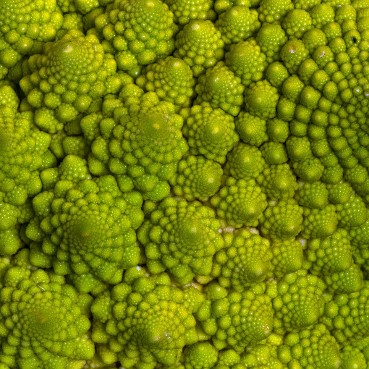
\includegraphics[width=\textwidth]{img/nat_pat_01.jpg}
		\caption{}    
	\end{subfigure}
	\hspace{10 mm}
	\begin{subfigure}[b]{0.225\textwidth}  
		\centering 
		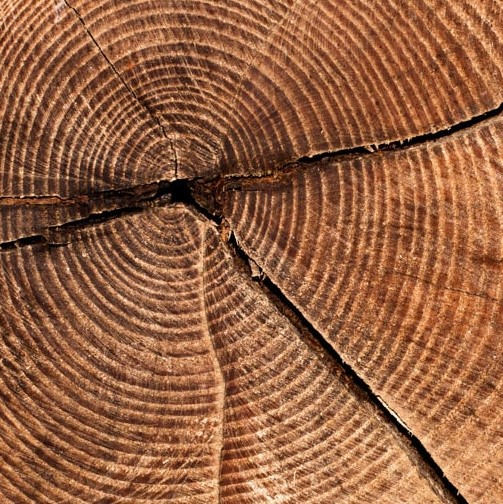
\includegraphics[width=\textwidth]{img/nat_pat_02.jpg}
		\caption{}  
	\end{subfigure}
	\vskip\baselineskip
	\begin{subfigure}[b]{0.225\textwidth}   
		\centering 
		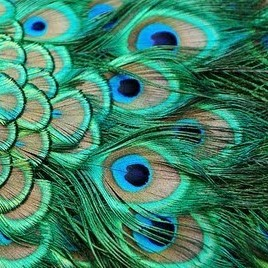
\includegraphics[width=\textwidth]{img/nat_pat_03.jpg}
		\caption{}    
	\end{subfigure}
	\hspace{10 mm}
	\begin{subfigure}[b]{0.225\textwidth}   
		\centering 
		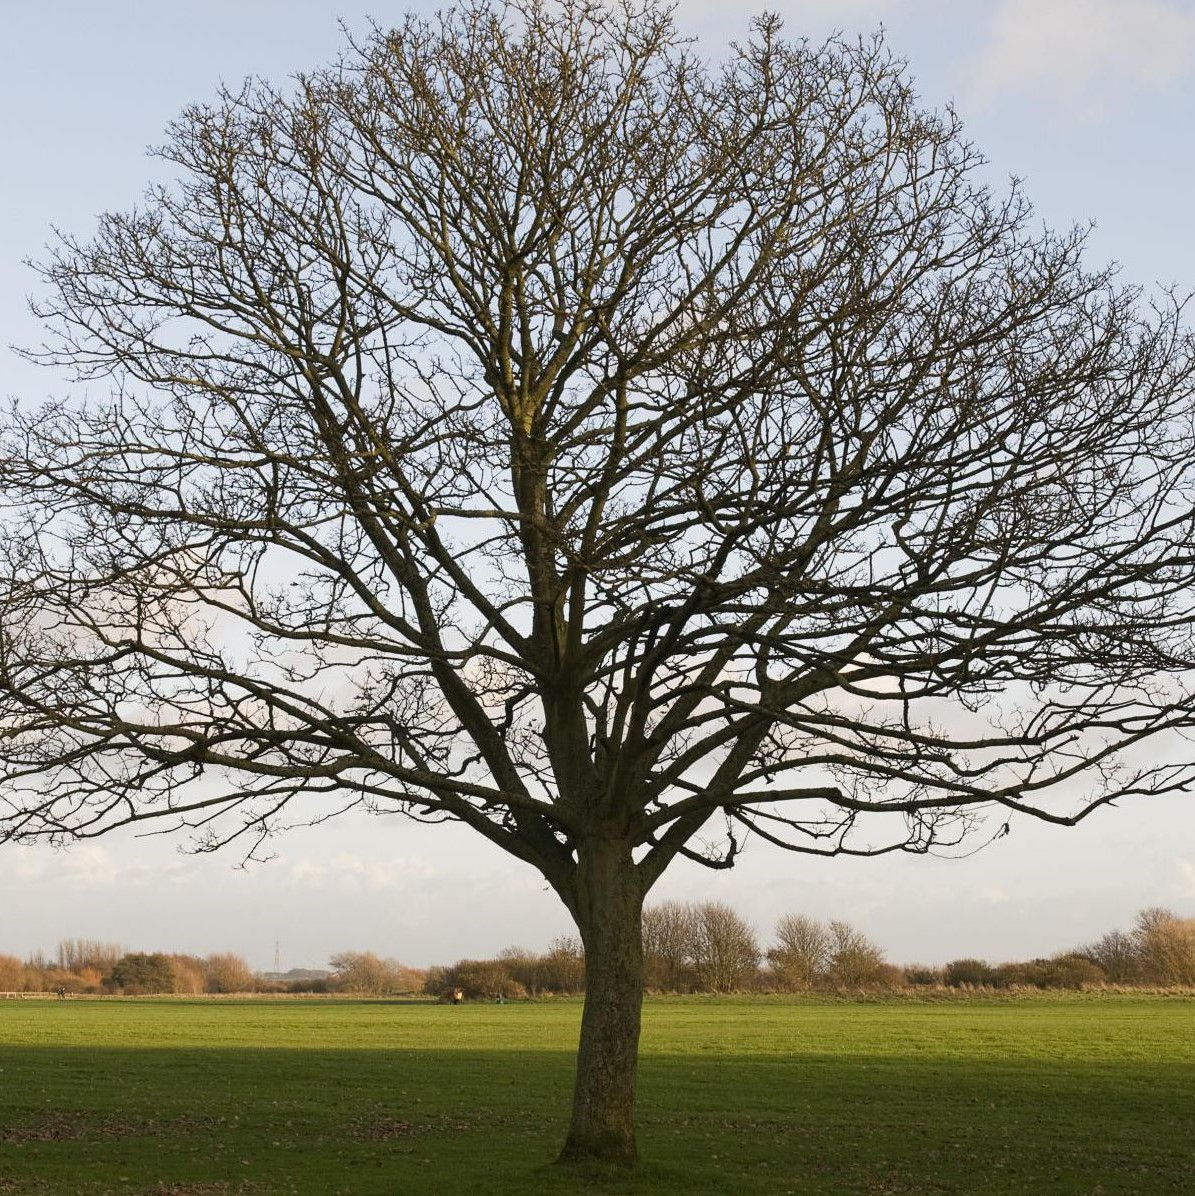
\includegraphics[width=\textwidth]{img/nat_pat_04.jpg}
		\caption{}  
	\end{subfigure}
	\caption{}
	\label{fig:nat_pet}
\end{figure*}

Mint ahogy azt Kovács Nemere is kifejti a A képzőművészet története III. részében az ősművészeteknél \cite{nemerekepzHomHuveszet} a természeti motívumok és eszközök már az ősidők óta részét képezik az emberi művészetnek. Amikor a barlangrajzokat készítették számukra az elsődleges forrás a természet volt, (\ref{fig:osi}. ábra).
Abban az időben az ember csak a környezetében található tárgyakat tudta felhasználni és az akkor kialakuló emberi kreativitás által az egyszerű eszközök és alapanyagokból létrehozni a művészetet. A saját tapasztalatuk útján jöttek rá, hogy miként tudják felhasználni az őket körülvevő anyagokat: növények, ásványok, rovarok és mindent amit megismert az elméjük. Az így megismert és létrehozott alapanyagokkal kezdték újrateremteni az érzékelt világot primitív művészeti formákban, például barlang rajzok, kezdetleges bőr művek vagy éppen primitív szövetek formályában. A legleső szín ami az ősi művészetekben megjelent a sárga és annak árnyalatai voltak, amit különböző növényekből tudtak elő állítani.
A nomád, vándorló népek napjainkig őrzik ez az erős természettel való együttélést. Színezékeik mind az őket körülvevő és épp aktuálisan megtalálható növényből készülnek.

\begin{figure}[h!]
	\centering
	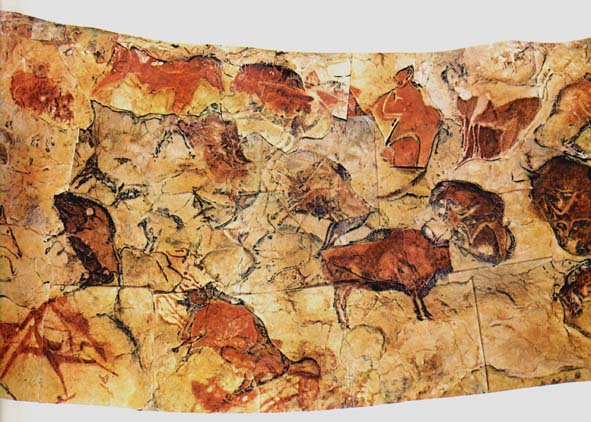
\includegraphics[width=0.5\textwidth]{img/osi.jpg}
	\caption{Barlang rajz}
	\label{fig:osi}
\end{figure}

Első ránézésre a természet néha egy kaotikus képet mutat magáról amit nehéz értelmezni, de az idő haladtával az ember elkezdete ezeket a kaotikus mintázattokat vizsgálni és értelmezni és rájöttek, hogy ebben a kaotikus képben valamelyest rejlik egy matematikai rend.

A természetben megfigyelhető minták, alakzatok, formák rendszeresek ismétlődők ilyen mintázatok a fraktálok (\ref{fig:fraktal}. ábra). A fraktálok egyik legismertebb tulajdonsága mint ahogy azt Mandelbrot Benoit B. is kifejti \cite{mandelbrot1982fractal} önhasonlóság, a természetben nagyon sok helyen találkozhatunk ilyen mintázattal, nem csak formai hanem rendszer szinten is nagyon jó példák erre a fák ők is természetes fraktálok abban az értelemben is, hogy sokszorosítják magukat és, hogy az erdő és természet létrehozza a biológiai önhasonlóságot. 

\begin{figure}[h!]
	\centering
	\begin{subfigure}[b]{0.4\linewidth}
	  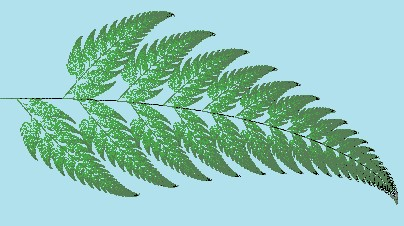
\includegraphics[width=\linewidth]{img/fraktal_01.jpg}
	  \caption{}
	\end{subfigure}
	\begin{subfigure}[b]{0.47\linewidth}
	  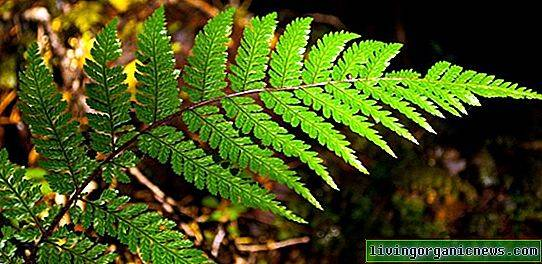
\includegraphics[width=\linewidth]{img/fraktal_02.jpg}
	  \caption{}
	\end{subfigure}
	\caption{Fraktálok és páfrány levél}
	\label{fig:fraktal}
  \end{figure}

A természetben persze nem csak ilyen mintázatok jelennek meg, hanem egyszerűbb struktúrák is mint például a foltok, a csíkok, a spirálok, a fodrok, az elágazás vagy a repedések, törések és a növények növekedése során lerajzolt formák is ebbe a körbe tartoznak.

Dolgozatom célja hogy megmutassam miként jelennek meg a művészeti alkotásokban a természeti minták és motívumok mint szerkezeti és strukturális szinten. Ezt egy technikán keresztül mutatom be, amelynek alapja a természetes alapanyagok, nevezetesen az indigó és a természeti motívumokból inspirálódik. 

\section{Alapfogalmak}
A dolgozat írás közben felhasznált alapvető és szükséges fogalmak:
\begin{itemize}
	\item \textbf{Motívum} \\  A művészetekben a legkisebb önálló kifejezőegység, amely a mű során általában ismétlődik. A folklór - népművészet alkotás legkisebb tartalmi egysége, amely átvétel után is felismerhető marad.
	\item \textbf{Organikus} \\ szerves, növényi , állati eredetű alkotóelem, 
	\item \textbf{Ornamentika} \\ (a lat. orno, 'felszerel, díszít' szóból): egy-egy kor, nép, műfaj vagy stílus díszítményeinek összessége. - Lehet mértani, növényi, figurális v. vegyes összetételű.
	\item \textbf{Festék} \\ Tágabb, köznapi értelemben mindenféle anyag, ami egy tárgy színét megváltoztatja: fedőfesték, máz, zománc, lakk, pasztell, lazúr stb. Szűkebb értelemben: a felületre felvitt, az alapot (szinte) teljesen elfedő, vékony, pigmentált réteg. A kötőanyagtól függően lehet: enyv-, olaj-, akril*-, tempera**-, viasz-, méz-, gyanta- stb. festék.
	\item \textbf{Színezék} \\
	Vízben oldható színezőanyag, mely kötőanyagot nem tartalmaz, jellemzően a kelmefestés kelléke. Az anyagot nem fedi el a színezék, hanem beleivódik a rostjaiba, a pigment kémiailag kötődik az anyaghoz. A létrejövő szín és teltsége függ a textilanyag fehérségétől, a kezelés időtartamától, a festőoldat sűrűségétől, az elő- és utókezelés módjától, anyagától (pácoktól*), ezek vegyi összetételétől, olykor más tényezőktől is.
	\item \textbf{Kelmefestés / Kékfestés} \\ 
	Egy textíliákon alkalmazott színmintázási technológia, amely nevét onnan kapta, hogy a minta eredeti formájában jellegzetesen kék alapon fehér színben jelenik meg.
	\end{itemize}

\section{A természet mint  inspirációs forrás}
A művészi kifejezőeszközök mentén az alkotó megfigyeli a természetet és gyakran lemásolja azt, mindeközben egy absztrakciós folyamat alá veti, mindeközben egyszerűsödik a természeti motívum, újraértelmeződik és adaptálódik megfeleő médiumra.
%A művészet utánozhatja a természetet azáltal, hogy egy absztrakción keresztül újra értelmezi azt, vagy képes teljesen lemásolni.

%A művészet kinyit olyan ajtókat nekünk a természet felé ami a természet  bonyolultságára és szépségére hívja fel figyelmünket, amit semmi képen nem lehet elszalasztani.

Lehet egy egyszerű művészeti kép ami segít értelmezi a természetet vagy lehet egy kihívást jelentő darab ami kifejezi a emberi kapcsolatot a természettel.\cite{art_nature} 
A természet megfigyelése mentén végbemenő gondolkodásmód által való művészeti  lehetőségeket  add nekünk egy olyan látásmód kialakítására ami maga a természetben előforduló anyagokkal, tárgyakkal való munkát helyezi a művészeti folyamat közép pontjába mint például levelek, botok, ágak, termések, víz, kövek és ezekhez hasonló természeti tárgyak használata.
Mindezek megfigyelése és azok tulajdonságainak értelmezése a design gondolkodásban is jelen van. Ezt nevezzük Anyagvezérelt tervezői gondolkodásnak vagy Material Driven Design-nak \cite{karana2015material}.
Kreatív módon való felhasználást késztetést érzünk új művészeti tárgyak készítésére.
\cite{meller2002textile}
Ez a fajta művészeti filozófia fenntartja a kapcsolatot az őskori emberekkel és a természettel. Transzcendentálissá és az időn átívelővé téve természetet, ember és művészetet.

Manapság sok kortás művész messze van attól a folyamtól, hogy ténylegesen saját maga hozzon létre bármilyen alapanyagot mint például festék vagy pigmentek a saját munkájának a megvalósításában. Ezzel ellentétben egyre kevesebb olyan művész és mester ember található aki a teljes alkotói folyamatot átlátja és végig vezeti.

\vspace{3 mm}
Egy ilyen kortás ritkaság a hagyományos japán kerámia a Tamba Yaki \cite{tambayaki}, ez az  egyik a 6 hagyományos fazekas stílusnak japánban, több mint 800 éves múltra tekint vissza. Egyik jellegzetessége a régió Kiotó és Oszaka között a Kurakura és a Wadajaki hegyek között elhelyezkedő hegyi falvak és az ott található alapanyagok. Ma is a mesterek maguk gyűjtik és készítik el a kerámiákhoz használt agyagot és mázat amit a mesterek saját titkos receptúrája alapján, de a legfontosabb, hogy csak is a régióból származó természetes összetevőkből állít elő. A kerámiák felületén kialakított minták és motívumok is a természetből származnak amit lenyomatolással levelek termések felhasználásával vagy festés - karcolás váltogatásával állítanak elő. Ez az irányzat az egyszerű és letisztult természetes vonal vezetéséről ismert, és hogy mindennapi használati tárgyakat állítanak elő. Az, hogy az ősi technikák formák és minták túlélték  a századokat és még ma is több műhely és mester dolgozik annak köszönhető, hogy mindig is lehetőséget biztosítottak a különböző művészeti határsoknak forma világoknak a beemelésére és a 20. század elején megjelenő Japán Kézműves mozgalomnak.

\vspace{3 mm}
Egy közismert mai kortás alkotó aki művészetében visszanyúl az ősi alapanyagokhoz Andy Goldsworthy. Olyan természetes anyagokat használt fel munkái során mint például levelek, kövek és hely- specifikus szobrokat készített amelyek tükrözik az anyagok és a természet közöti ősi kapcsolatot.

Munkáinak az elkészítési ideje hosszú folyamat, a felhasznált  alapanyagok össze gyűjtése és előkészítése mélyíti el azt az ősi kapcsolatot ami művész és műalkotás között ki tudd alakulni.
A kész művei fényképformájában maradtak fent mivel ezek az alkotások a természetben helyezkednek el és semmilyen olyan alkotó elemet nem tartalmaztak ami megóvná a természet viszontagságaitól és lassan elamortizálódtak ilyen módon fejezte ki, hogy a tényleges műalkotás múlandó.

% \section{A természet a magyar kortás művészetben}

% Ide bármilyen kortárs magyar művészt aki valamilyen természet közelit csinál.

% \subsection{Színanyagok}
% A természetben előforduló pigment anyagok melyek felhasználásra kerülnek a legkülönfélébb művészeti alkotásokban:
% Indigó, Bíbor, 
% \subsection{Eszközök}
% Nyomódúc. textilminták előállítására használt fa mintanyomó eszköz, leginkább puha és keményebb fa fajtákból készült mint például gesztenye fa vagy dió fa vagy tölgy vagy bükk
\section{A természet a saját mintáimban}
Az eddig munkáim során a ösztönösen a természetnél lyukadtam ki, de miért pont a természetnél azt még az elején magam se tudtam, ahogy elkezdtem a különböző feladataim során a tanulmányokat mindig a fák és terméseik lettek a fókuszban e fafajták közül hármat választottam.

Próbáltam olyan természeti elemeket keresni, amik a minden napi köztudatban benne vannak és ezeket a természeti formákat mindenki ismeri és találkozótt vele és már felhasználta ezeket valamiyen formában. 

Ezek a termések a dió, a makk és a gesztenye volt \ref{fig:sajat1}. ábra.
Ezeket a terméseket szeretném egy újabb, modernebb irányban vinni ahol ezek a természeti elemek más arculatban, könnyed vonal rendszerrel, de mégis felismerhető minta ként jelenjenke meg az emberek számára.

\begin{figure}[h!]
	\centering
	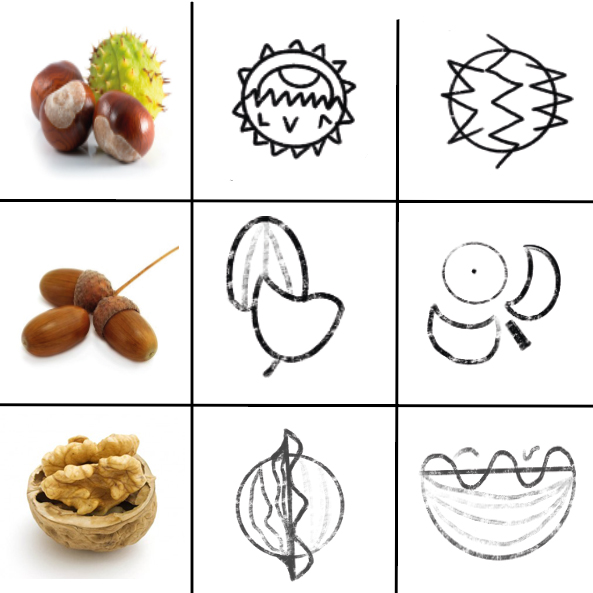
\includegraphics[width=0.8\textwidth]{img/sajat01.jpg}
	\caption{Saját mintakészlet fejlődés. Gesztenye - Mak - Dió}
	\label{fig:sajat1}
\end{figure}

\chapter{Az indigóval való festés}
Az indigó név Római indicum -ból származik ami Indiai terméket jelent.
Ez a megnevezés bizonyos értelemben téves név mert az indigót tartalmazó növényeket a történelem során a világ több pontján is termesztették, mint például Kína, Jáva, Japán és Közép-Amerika.  

Az 13. százelején amikor Marco Polo haza érkezet ázsiai utazásáról, amelynek során rájött, hogy az Europában hőn áhított és nagyon kereslet indigó nem egy ásvány hanem egy növényekből származó festékanyag és magával hozott egy palántát új színtörtbe az Európai divatba. Ezt követően már Európában is beszerezhetővé vált.

Majd a 16. században Portugália és Spanyolország bonyolította le az indigó kereskedelem nagy részét, mondhatni Indigó nagyhatalmakká lettek.
Ezt követően a Hollandok sajátították ki maguknak mert elkezdték nagyobb mennyiségben szállítani az indigót köszönhetően a modernebb és fejlettebb hajó flottáiknak. Ennek következményeként tönkre ment az Európai csülleng termelés. A legjelentősebb mennyiség gyártást Indiában kezdték el 1600 évek végén sok indigót hoztak be Európa.
 
\section{Technologiája}
 \textbf{Növényi indigó}
 Europában az indigó előállításánál festőfűként nevezett (festő csüllenget) használtak elsődlegesen. Ez a egy kétnyári fű fajta ami az év első felében levél szerű rozettákat nőveszt.
 Amikor az indigót kezdik el termeszteni, akkor learatják ezeket a rozetta szerűségeket. A következő évben virágkocsányokat és magokat hoz létre.
 A középkor tájékán fontos gazdasági szerepe volt a festő fűnek Europában, ez hozta a legtöbb jövedelmet.  
 A hagyományos indigó festék előállításánál a festő fű leveleit péppé zúzták labda formákat készítettek belőlük ezeket több hétig szárították és ezt majd egy fermentációs, erjesztési folyamat követte majd a feldolgozás további lépéseiben is többször újra és újra össze zúzták. \cite{tiborindigokemia}
 Sajnos a festő fű nagyon szennyezett volt, és ezért csak egy nagyon halvány kék színt tudót adni.
 Ezzel ellentétben a trópusokról származó indigó sokkal jobb minőségű volt és mélyebb gazdagabb kék színt hozott.
 A növényi anyag kapott egy vizes áztatást, utána elkezdték az erjesztési folyamatot és ezt követte a levegőn történő oxidációs folyamat. Maga a növény nem tartalmazta az indigót, hanem azokat az alap vegyületeket melyek a fermentáció során átalakulva hozzák létre a kívánt pigmentet.

\section{Földrajzi varianciája}

\subsection{Magyarországon}

Magyarországon a 18. század közepétől volt elterjedve ez a mesterség.

A Nyugat-Magyarországon lévő manufaktúrákban egyre több külföldi munkás fordult meg, ezen részén az országnak nagy fejlődés vette kezdetét .
A 18. század tájékán Mária Terézia idején kezdődött el Magyarországon az indigó és csülleng fű termesztés.

Azért próbálkozott Magyarország a termesztéssel mert szerették volna csökkenteni az Európát elárasztó indiai és türingiai festéket.
Ebben az időben komoly gazdasági alapja volt Magyarországon, több mint 300 falu foglalkozott a csülleng fű termesztésével  és feldolgozásával.
Néhány vidéki városban a 19. század idején az ottani igényeket figyelembe véve készítették el a termékeket legyen akár szó lakástextilről vagy egyéb felhasználásról.

\subsection{Európában}
A kékfestett textil kereskedelem fő központja 18. században Franciaország  és Németország volt.

\vspace*{3 mm}
Franciaországban a kékfestést technológiája eltért a többi Európai országhoz képest. Az ottani módszer jobban hasonlított a batikoláshoz. A textilanyag felületét viasz réteggel vonják be, arra a részre ahol nem szeretnék, hogy befogja a festék és ezzel a módszerrel sokkal tisztább és élesebb dekoratív mintákat tudtak elérni ennek a viaszos alkalmazásnak a segítségével.
Mintakincsük sokkal aprólékosabb részlet gazdagabb inkább levélszerű mintákat alkalmaznak, ezek közt elvétve fel tűnik egy két virág motívum mely apró és elhanyagolható a teljes mintában.
A minta fa készítéshez gyümölcs fa fajtákat használtak fel mert sokkal lágyabbnak és puhábbnak tartják a véséshez és kaparáshoz. Az általuk előállított anyagok több színűek és esetenként a minták is színesek.
Például a vörösszín eléréshez festő fűt alkalmaztak a festő buzér - Garance - Rubia tinctorum  ez a nővény alapozta meg a vörös szín használatát, 
a sárga és a zöld szín előállítása a festő csülleng feldolgozásának részfolyamatainál mint melléktermék jött elő.

\vspace*{3 mm}
Németországban három technológia volt elterjedve a Tartalék (Reservedruck), közvetlen (Direktdruck), maratás (Ätzdruck). Az alap textilt először fehérítették, szárították és végül hengerelve (Mangeln) vasalták és keményítették.

A tartalék nyomás során fehér mintát hoznak létre kék alapon. Az eljárás során a gumiból hozzák létre a nyomatot. Ezt követően a nyomatot (Reservage) bevonják egy festék taszító anyaggal és a minta nyomás száradást követően történhet. A festék összetétele: fehér dohány, réz-szulfát, réz-acetát és egéb titkos összetevők. Pasztell vagy német indigónak hívták ezt a festéket. A festés után a mintát hígítót kénsavval távolítják el.

Ezért ez egy festési eljárás, nem egy nyomtatási folyamat. A "tartalék" kifejezés arra a tényre utal, hogy a kiválasztott minta a festés során kimarad.

A közvetlen nyomtatásban a színt az előkészített fehér szövetre nyomtatják a nyomdarúddal. A szín közvetlenül az anyag felületére kerül, és barna színként jelenik meg. A száradás után a szövet egy fürdőbe helyezik, amelyben a barna tinta kémiai reakcióval élénkkékre változik. A szövet végül felfőzik, újra hengerlik, ezt követően használatra kész. A nyomtatást nagyon óvatosan kell elvégezni, mivel a hibákat nem lehet kijavítani.

A maratás folyamata egy kék színű alap szövet is nyomtatható maró anyaggal (maró folt), ami kék alapon fehér mintázatot hoz  létre. Ez a technika alapvetően Hollandiából származik, de máshol is elterjedt az eljárás.

\subsection{Ázsiában}
A Shibori egy a 8. századból származó japán textil festési technika \cite{shibori} amelynek lényege, hogy különböző kötözési, csomózási eljárásokkal állítanak elő tetszőleges mintázatot.

A Shibori számtalan más japán alap technikát foglal magában, iylen technikák például a miura, a kumo, a nui, mindegyikben közös, hogy valamilyen kötözési módszer vagy az anyag hajtogatást alkalmazz. 

A kötözés és hajtogatás mellet a szövetett olykor festéktaszító anyaggal is bevonják és ezzel is mintákat hoznak létre.

A teljes minta elő állításának folyamata az alap szövet tisztításával és esetleg fehérítésével kezdődik, ezt követően történik a vasalás és hajtogatás vagy a szövet összefogása és kötözése és felületének kezelése.
Az Shiboriban az, hogy milyen technikát használunk nem csak a saját preferenciánktól függ vagy a vágyott mintától, hanem a befestendő anyag tulajdonságaitól is. Ezen kívül  a különböző festési módszerek kombinálhatunk kidogozottabb, bonyolultabb, részletesebb minták elérése érdekében. 

\subsection{Különböző régiók összehasonlítása}
   Az országok közötti hasonlóság elsősorban az, hogy ugyan azt a festő nővényt használják fel a munkájuk során.
   De technikailg a minták előállítást is más kép működik,és ezért nehéz a minták kőzött hasonlóságot keresni , de a  minták  elkészítéséhez valamilyen téren a természet által inspirálódnak , míg az egyiknél teljesformájában jelenek meg a természeti minta elemek másik részéről még vonallak vagy pontok , körök formájában jelenek meg a minták  
    igazából a minták elkészítés mind a két téren finom érzéket és türelmet igényel.

\chapter{A kékfestés}
\section{Előzménye és történelmi áttekintése}
Kékfestészet előzményének a kelmefestészetet, és a textilnyomást tartjuk ami egyszínűre színezést és mintázást jelent mely technológiák már a 15. - 16. században is léteztek. Sok tudást igénylő művészeti ág volt.

A középkori kelmefestés kezdetekben a városokban és a kolostorokban működtek különféle anyagok színezésével foglalkoztak mint például gyapjú vagy vászon. 

Az indigó megjelenéséig Magyarországon a kelmefestésre a festő csülleng növényből elő- állított kék festékanyagot használták. Ez a 15. században  kerül Magyarországra és terjedt el fő alapanyagként.

A csülleng fontos szerepet töltött be a középkortól kezdve, legnagyobb termelő területek Franciaország és Türningában volt. A magyarországi mestereknek a beszerzési központ Türnigiában volt.
A 16. század körül körülbelül 300 falu foglalkozott a csülleng termesztéssel Magyarországon. Aki akkoriban a csülleng termesztéssel foglakozott vagyonosabb réteghez tartozott. 

A 17. századra visszaeset  a termesztés mert ekkortájt a holland hajókaravánok behozták kelet Indiából az indigót.Ezekben az időkben már csak körülbelül 30 falu foglakozott még a termesztéssel.

Az 1600-as évek körül Brassó város könyveiben jelent meg az első feljegyzés a posztó kereskedelemről.
Létezett egy céhen kívüli szervezet aki szétosztotta  a mesterek között festendő posztót \cite{domonkos1981magyarorszagi}(14-17).
Miután a mesterek elkészültek a festetett mintás anyagokkal azokat a céh újra összegyűjtötte és kereskedtek  velük más városokban vagy exportálták Európa különböző részeire.

A 16. -17. században az ország még török fenhodltság alá nem esőrészén az ország északi területei hirtelen és hatalmas fejlődés vette kezdetét.
Az elfoglalta területekről menekülők elárasztották az ország északi városait és egyre nagyobb lett a zsúfoltság és a népesség amit az akkori mesterek kihasználtak, de a műhelyek kicsik voltak és a sok munkástól egyre zsúfoltabbá váltak, ez a termelés és a gyártás kárára vált már ekkor.

A kisvárosokban mint például Lőcse, Eperjes itt már a 16. században több mester  fogalakozott anyagok és fonalak  festésével. 

Nem csak a dolgozni vágyó munkások indultak meg a déli országrészről hanem az onan menekülni kényszerülő mesterek is. Ezek a vándorló mesterek új Céheket hoztak létre, bizonyos esetekben a helyi mesterekkel közösen vagy konkurenciaként a már meglévőkkel szemben. 

Az első magyarországi feljegyzés a kékfestésről 1783-bol van Körmöcbányáról, a 17.század közepétől indult meg a kékfestészet elterjedése meghonosodása Magyarországon  %referencia kell erre

A 18. században szinte minden városban volt olyan mesterember aki ezzel foglalkozott az igen nagy kereslet miatt. Egyre nagyobb kereskedelmi igény alakult ki a nyomot mintás anyagok iránt sok mester próbált új technikákat létre hozni, illetve  elsajátítani a más régiókból származókat, hogy ezzel kiemelkedjenek a már meglévő minták és anyagok sokaságából.

Sopronban volt a Boór család akik a 19. században, az egyik legfontosabb szerepet töltöttek be ők voltak az első mesterek akik ipari jellegű, gyárszerű  kékfestő üzemet működtettek.
1852 és 1861 között elkezdték a bővítést, és a későbbiekben külföldre is exportálták termékeiket Európa minden pontjára. Hatalmas gazdasági és kereskedelmi előnyre tettek szert a kialakított gyártás technológiának köszönhetően, sokkal alacsonyabb előállítási költséget tudtak elérni. A megnövekedett bevételnek köszönhetően Indiában béreltek földeket ahol saját maguk termesztették indigót.
A Goldberger (Kelenföldi Textilgyár - KELTEX), és a Felmayer (szegedi műhely) is, külföldi tapasztalatok alapján végezte ezeket a  munkafolyamatokat a 19. század közepére mindenhol Ipari méretekben ment már a kékfestés és a kelmefestés.
Amikor megtörtént ez a nagy ipari fejlődés a hagyományos manufakturális céhes kisüzemek elkezdtek tönkre menni és ennek a kézműves iparnak a végét jelentette még körü belül 100 évig sikerült fentartanija magát de ezt követően nagyon kis számban maradtak fent műhelyek és mesterek akik a régi technikákat és módszereket tovább tudják adni és tanítani.
Az ipari fejlődés mellette a divat is megváltozott a vidéki életformák változása után a városi dolgozóknak az öltözködésük is meg változott a régi hagyományos viseletek igényei is változni kezdtek Magyarországon.
Az első és a másodig világháború után nyersanyag hiány lépett fel városiasodás tovább csökkentette a műhelyek számát.
De még egy két vidéki helyen ma is foglalkoznak és viszik tovább ezt a mesterséget próbálják fenttartani, hogy ne veszen el a kékfestészetnek a varázsa.

\section{Technológia}
Egy kékfestő műhely létrehozásához is jelentős tőkebefektetésre van/volt szűkség, egy teljesen külön álló épület szükséges hozzá az oka ennek hogy a kékfestés eljárás során sok veszéjes egymással reagálni képes vegyszert használtak és ezek elkülönítése és tárolása egy fontos igény. Szükséges egy helység a színezésre és a kifőzésre, a  kifőző helységet fekete konyhának hívták nevével ellentétben ez egy álltalában fehérre meszelt sok kádas helységvolt. A minta készítés is egy külön helységeben történik amit a küpa szobának hívnak. A szárítás általában az udvaron történik, száritó egy az udvar közepén lábakon álló vagy az épület oldalára erősíttet gerendázat (\ref{fig:udvar}. ábra), rosszabb idő esetén ezt akkor bent a műhelyben  kell valahogy kivitelezni.

\begin{figure}[h!]
	\centering
	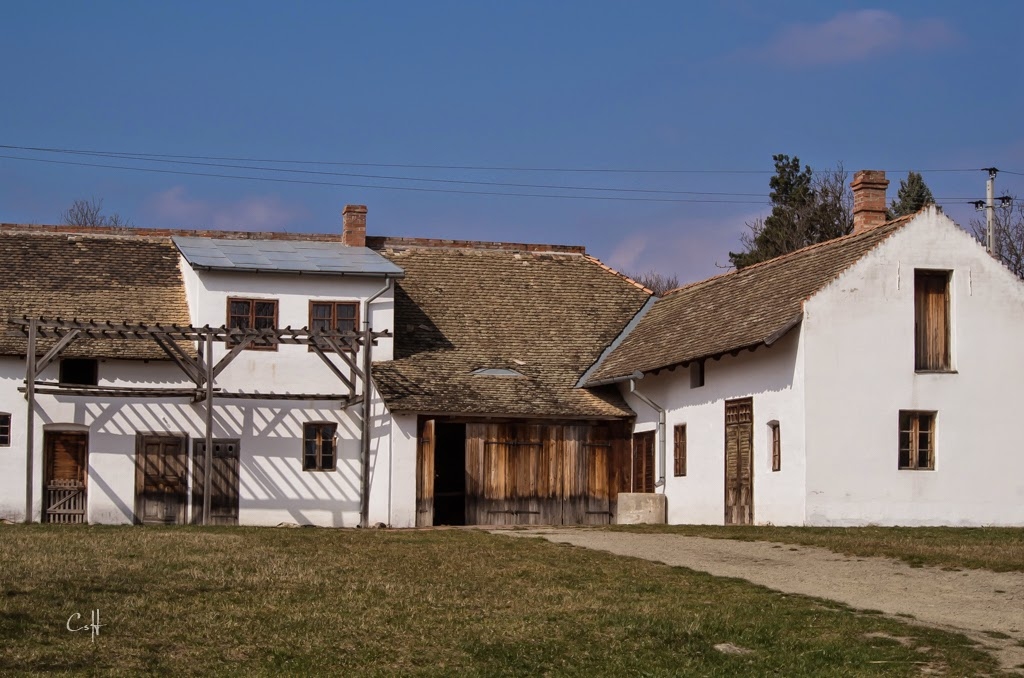
\includegraphics[width=0.5\textwidth]{img/udvar.jpg}
	\caption{Kékfestő műhely , udvar, szárító gerendák}
	\label{fig:udvar}
\end{figure}

Ezek a műhelyek általában a családi telkekre épültek. A az ipari mennyisségben gyártó nagyobb műhelyek kőrű belül 4-5 katlannal rendelkeztek. Az első fő lépés a vásárolt vásznakat kifőzték a szennyeződések miatt, másfél órán keresztül szódás vízben. Miközben ment a kifőzés, keményítős oldalát megjelölték nehogy arra az oldalára kezdjék el a mintázást, mert sajnos akkor az anyagon nem tud rendesen megmaradni a minta és foltos lesz. A  fentmaradt végeket a fekete konyhába vitték és egy literes fa kádban tiszta vízben kiöblítették őket. Miután befejeződött a öblítés jött a száritás. A szárítás kültéren vagy beltéren történik attól függően milyen az idő, ha fagyos időben kint száradtak az anyagok akkor a keményítő a hideg hatására elszineződött és rontotta a végtermék minőségét és esztétikumát az ilyen anyagokat már nem tudták felhasználni és bekerült a selejtek közé, ebben az időszakban szüneteltetniük kellet a munkát ez körű belül 6 hónap kimaradás volt a részűkről. Igy akkor kevesebb munkásra volt szűkségük, de addig az úgy mond pihenő idő alatt sem tétlenkedtek hanem a minta dúcokat tudták előkészíteni.
A századforduló idejére már több vidéki műhely is rendelkezett gőzgéppel vagy kazánházzal ezeknek a segítségével már betudtak szerelni télire szárítókat a műhelyen belülre is \cite{domonkos1981magyarorszagi}(40-48).
A kézi mintanyomás egy párnázott asztalon készül, amire több rétegben pokrócokat helyeztek majd a végén molinóval befedték, az asztal felületét úgy lehetet elképzelni mint a pecsét párna lenne, igy az asztal felülete nagyon puha lett.

Búzát, kukoricát, burgonyát alkalmaztak az anyagók keményítésére, ez a folyamat a fekete konyhában történt. A megszáradt végeket elvitték a mángorlóba, ez a szerkezet  egy erős gerendára szerelt asztalalapzatból állt rajta erős vastag keményfa, görgőkön mozgott, mérete körű belül 4-6 méter hosszú lehete és körű belül két és félméter magas, akkoriban ezeket lovakkal hajtották. Kapcsolódott hozzá egy láda, a fölött elhaladt egy főtengely és amire került fel egy vastag lánc ami az asztalon lévő ládát mozgatta.

A belső kerekeknél két főtengely helyezkedett el váltókar segítségével lehetett irányitani ezzel azt tudták elérni, hogy jobbra és balra is tudták forgatni a szerkezetet. A legfontosabb az volt hogy kis helyen is elvéghető legyen ez a munka folyamat. A fokozódó verseny helyzet miatt az ipariméretekben gyártókkal olykor előfordult vissza eset a kisműhelyek forgalma és akkor sajnos nem volt pénz lóra aki hajtsa a kereket akkor maga a mester álltbe és tekerte a szerkezetet. A mángorló több változta is létezik (\ref{fig:mangorlo}. ábra) az általános méret 30x30  ezeket a szerkezetek általában vastag gerendákból építették fel 15-20mm vaslemezeket szereltek fel rá.
Azokba a műhelyekben ahol adott volt a gépesítés ott gőzgép vagy transzmissziós tengelyekkel vitte az erőt a mángorlóba ezt a technológiát Pápán, Csornán és  Békéscsabán használták.

\begin{figure}[h!]
	\centering
	\begin{subfigure}[b]{0.2\linewidth}
	  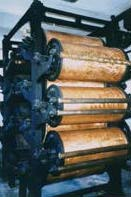
\includegraphics[width=\linewidth]{img/mangorlo.jpg}
	  \caption{}
	\end{subfigure}
	\begin{subfigure}[b]{0.3\linewidth}
	  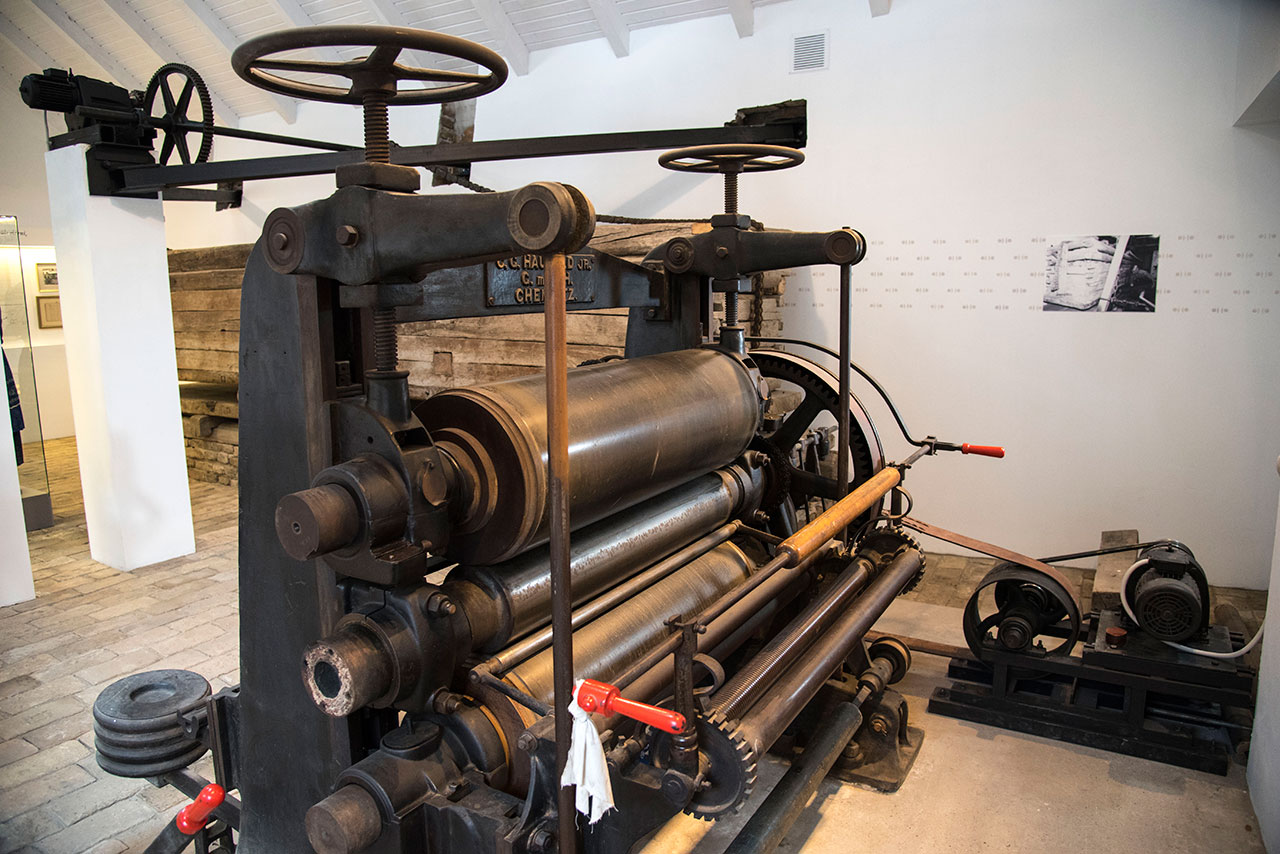
\includegraphics[width=\linewidth]{img/20.jpg}
	  \caption{}
	\end{subfigure}
	\begin{subfigure}[b]{0.3\linewidth}
		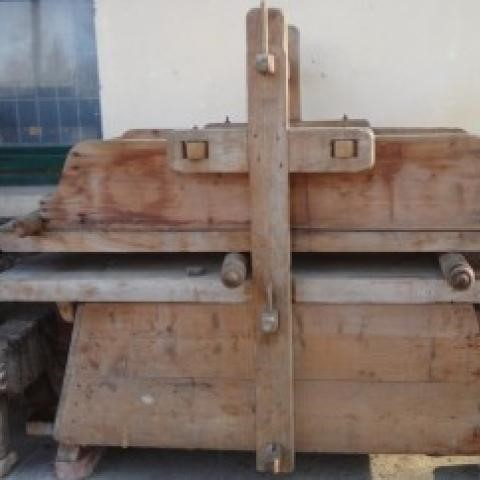
\includegraphics[width=\linewidth]{img/28613.jpg}
		\caption{}
	  \end{subfigure}
	\caption{Mángorlók}
	\label{fig:mangorlo}
  \end{figure}

Más városokban például Bátaszék, előfordult a technikai fejlődésnek köszönhetően, hogy benzinmotort alkalmaztak, vagy mint például Csornán villany meghajtásura építettek át a mángorlót. Fontos fő alkatrésze a mángorlásnak a görgő és az áruhenger volt. Az únt felhelyezték a felsodrószékre és a vászon végét beburkolták. Miközben mozgásban volt nagy súly volt rajta, és ide oda mozgott eközben kisimította az anyagot. Mielőtt elkezdődött a mintázás kétszer háromszor végezték el ezt a folyamatot, a festés után a keményítés körű belül hat - nyolc  vagy akár tíz alkalommal is elvégezték. Maga a mángorló téglával lerakott helység volt itt készítették el a vegyszereket is. 
A minta készítésnél használt fő fedő anyag az a pap volt álltlában más - más összetételben készült ez anyag nagy titkos receptek alapján készítették el és, hogy több hónapig elegendő legyen így egyszere egy nagy mennyiséget készítettek el.  Ahhoz hogy ne mennyen tönkre ez az anyag nyirkos hűvös helyen tartották. A papot különböző  pácokhoz és fedőanyagokhoz is hozzá keverték, mikor megkezdődött a kék festés akkor mész lúgos öblítéssel sárga, zöld, narancs színű mintákat is tudtak előállítani.

Nálunk nem volt megszokott a  színes mintás anyagok készítése mi maradtunk fehér minták létrehozásánál, ez a stílus inkább a franciák körében volt jellemzőbb. A mintázáshoz is volt egy külön helység amit használtak és ott abban a helységben volt a tarkázó asztal, ez mellet helyezkedett el a Sasi.
A Sasi egy olyan láda volt ami körülbelül 6-8 cm mélységű volt, és egy sűrű keményitő oldat volt benne. A ládában volt egy keret aminek ez egyik oldala viaszos vászonnal volt bevonva a másik része pedig monílóval, ebben kenik el a fedő masszát a papot és kürűl belül úgy működik mint a pecsét párna.
A minta készítés nyomódúcokkal folyt, méret különbségek voltak a dúcok között, de ahhoz hogy hatékonyabb legyen mintás anyagok készítése nagyobb dúcokra kellet válltani de azoknak az elkészítési ideje sok időt vett igénybe igy átváltottak egy úgy nevezett perrotingépre ami  felgyorsította a gyártást. Az 1860 -as évek körül bekövetkezett egy nagy mértékű gépiesítés igy egyre több műhely állt át a gépi nyomásra.

\subsection{Folyamat}

A kékfestészet munkafolyamata úgy zajlott le egy műhelyben, hogy a nyersanyagot nem maguk állítottak elő hanem magánszemélytől vásárolták,  vagy maga a megrendelő vitte magával, eztkövetően a megrendelő kiválasztotta a mintát a minta könyvből. 
Voltak olyanok akik nem foglalkoztak mással mint a nyers alapanyagokat szerezték be a festő mestereknek.

Az első fő lépés az alap vászonnak a megtisztítása, ez egy kétórás folyamat ami alatt a szövetett egy szódás vizben mossák ki. A szódás kifőzést során az anyagból kioldódik egy gyantás anyag ami meggátolná a meg színezést és ez a folyamat után az anyag még ki is kifehéredik.

A mosást követi a hideg vizes öblítés és a szárítás ezek a folyamtok néhány órát igényelnek \cite{kisteleki}(107-113).
A száradást követően kap a már tiszta fehér anyag egy vékony keményítést ami előkészíti a mintázáshoz vagy más éven "tarkázáshoz".

Tarkázásnak említett kézi minta készítés párnázott asztalon készül.

Az asztal mellet helyezték el Únt és az ún-ba mártották bele a minta dúcokat.

A viaszkosvászon belső felületére kent fel a mintaázó pépet az Ún ládát feltöltötték sűrű keményitővel ami a sasit puhán tartotta. Amit általában használunk hozzá fehér nyomó pép, annak alkotórészei ólom-nitrát, ólomacetát, gumiarábikum, kék timsó, rézgálic. Ezeket össze főzik és miután ki hűlt egy hétre rá használják csak fel. A festék pépet maga a mester szokta elkészíteni általában ez a festék pép akár évekig is elég szokott lenni. A mesterek azt gondolják, hogy egy pép minél régebbi annál fehérebbé teszi a mintát.

A kékfestő a minta dúcot a nyomópépbe nyomja, majd és a dúcot a vászonra illeszti pontosan nehogy elcsúszon és erősen lenyomja, hogy minden pontra kerüljön a pépből és azt a részt nem fogja be a kék indigófesték. A mintázás nagy figyelmet és türelmet igényelt. Általában a kékfestők, 120-130 méter anyagot mintáztak meg, de az napi 13-14 órás munka folyamat \cite{kisteleki}(107-113).
Miután a minta nyomás befejeződött pár nap volt még megszáradt a nyomatás ezek után következet a festés.
Az anyagot egy ráfra akasztják,  ami egy vaskerék és erre akasztják fel az anyagot. Ez tehát úgy néz ki az anyag esése  miatt mintha vaskereken egy rakott szoknya lenne.
Következő teendő pedig, hogy elkezdték belengedni  az indigó festékkel teli kádba és félóránkként fel és le mozgatják az anyagot, és körülbelül 5 - 10 percet hagyják a levegőn hogy az indigó oxidálódjon.
Amikor elsőnek felhúzzák az anyagot a festékből akkor először egy sárgás - zöld színe van egy kis idő  múlva a levegő oxidáló hatására miatt egyre sötétebb zöld színe lesz az utolsó előtti merítés után már világos kék színe van. Miután egyre többet éri a levegő megkapja azt a szép sötétkék színt amit indigó kéknek nevezünk. 

Miután az anyag elérte a kívánt színt akkor következik a száritás. Miután meg száradt az anyag akkor kap egy kénsavas fürdőt ennél a folyamatnál az történik hogy kioldódióik a mintázásnál bele ragadta nyomópép és ezek után nagyon szépen elő jön a minta. Utána egy sima vízben is ki öblítik és hagyják megszáradni, és végül ki keményítik az anyagot.

Ez a teljes munkafolyamat valósítja  meg azt a fajta mély indigó kék szint ami lehetővé teszi a kontrasztot a minta és a festés között.


\section{A természet mint inspiráció}
\section{Minta dúcok}
Maga a minta és a forma készítés rajztudást igényelt és a textilnyomáshoz való ismereteket, a mintáknak mindig pontosan kellett egymáshoz illeszkedniük, ezt a készítőnek mindig szemelőt kellett tartani.

A nyomódúcok felületei általában mindig kiemelkedtek és negatívba kellett rajtuk a mintákat elkészíteni. Két fajta minta dúcot különböztetünk meg, az egyik fából kifaragott a másik pedig réz lemez formájú mintát. A mintadúc készítésének első lépése az hogy ha fából faragják ki a mintákat akkor kirajzolják a mintafára és utána azt elkezdik kifaragni. 

A kezdetekor úgy nevezték a kézi minta rajzokat mint például ágas, ágasindás, ágasvirágos, csokros, cakkos, folyondár, margarétás, négyzetpontos,akkoriban nagyon egyszerű neveket adtak a kész mintáknak. A kedvenc és bevált mintákat, idomait a perotinra a mintázó gép nyomó fáira is átvitték (\ref{fig:perotin}. ábra).

\begin{figure}[h!]
	\centering
	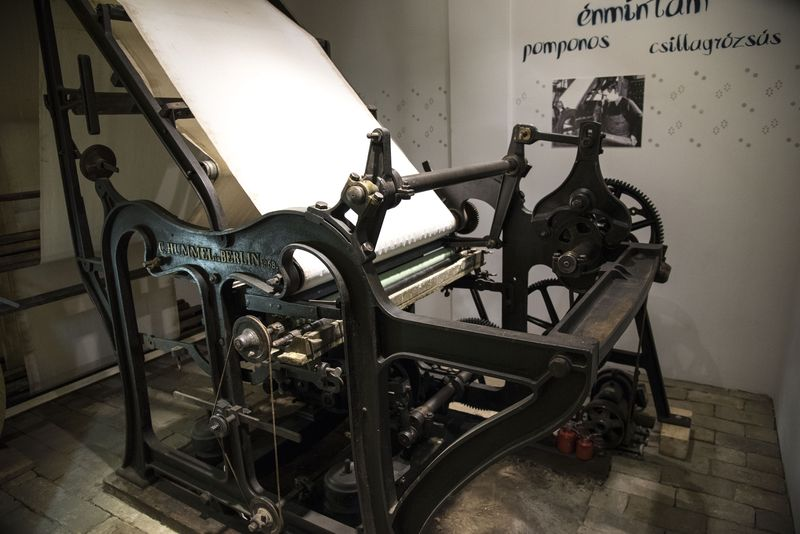
\includegraphics[width=0.5\textwidth]{img/201603-perrotin.jpg}
	\caption{Perotin}
	\label{fig:perotin}
\end{figure}

A 17. század és a 18. századi minta dúcokon pozitív nyomást alkalmaztak amikor növényi vagy figurális mintákat készítettek ezeket a metszeteket fadúcokra készítették. Ebben az időszakban már szinte minden városban volt egy minta készítő mester.

A 18. század közepe táján csak a Sasvári, a Cseklésziek minta készítő műhelyek vagy másnéven manufaktúrák  voltak az országban akik több mintakészítő mestert alkalmaztak azért hogy minél gyorsabban el tudják készíteni a mintáikat, a munkások még az itteni munka mellet tudtak foglalkozni vidéki műhelyek mintáival de miután végeztek mentek is vissza. 

Ez időtájt nem csak a hazai mintakészítők voltak jelen hanem egyes műhelyek külföldről hívatták a mintakészítő mestereket akiket a mintatervezés idényére elszállásoltak, ezt a luxust csak a gazdagabb műhelyek engedhették meg maguknak, ha a külföldi mester végzett a megbízatásával akkor már ment is tovább a következő megbízóhoz az újjabb munkákért erről olvashatunk \cite{domonkos1981magyarorszagi} (57-67).
Miután egyre jobban elkezdtek terjedni a nyomot kelmék igy vidéki műhelyek mintakincsei is egyre felkapotabbá kezdtek válni.

Későbbiekben létrejött nagyobb gyárak mint például Goldberger és Spitzer, Gerson és a Szegedi Felmayer ők alkalmaztak mintafaragó és készítő szakembereket.

A legelső minta fák teljes mértékben fából készültek kisebb pontok, ágak, hasonló képen mint a folt felületek, de ezeknek a készítésére legalkalmasabbnak a dió fát tartották vagy a körte és gesztenye fát mert ezek a fajták nem szálkásodtak egyszerű volt ki faragani belőlük a mintákat, tartósak voltak és nem repedeztek ki a nedvességtől.

A 16. század idején néhány nyomó dúcok kőzött előfordult tölgy és bükk is ezeknek használatával sok változás jött elő ugyan is ezeknél kezdték el használni a réz drótot, de későbbiekben már teljes mértékben vörös réz drótot használtak, azért volt jobb csak a vörös réz drótot használni mert az előállítása olcsóbb volt és így több mintát tudtak elkészíteni (\ref{fig:duc}. ábra).

\begin{figure}[h!]
	\centering
	\begin{subfigure}[b]{0.2\linewidth}
	  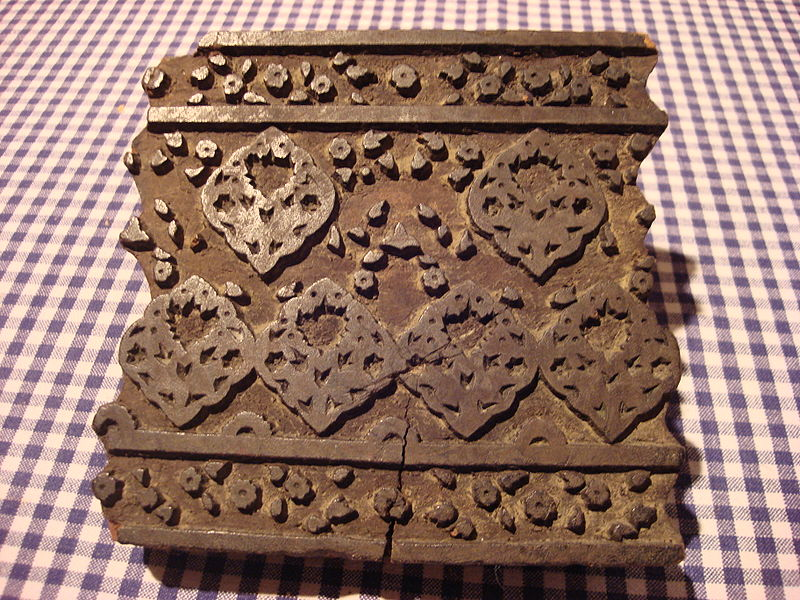
\includegraphics[width=\linewidth]{img/fábolkészült02.jpg}
	  \caption{}
	\end{subfigure}
	\begin{subfigure}[b]{0.2\linewidth}
	  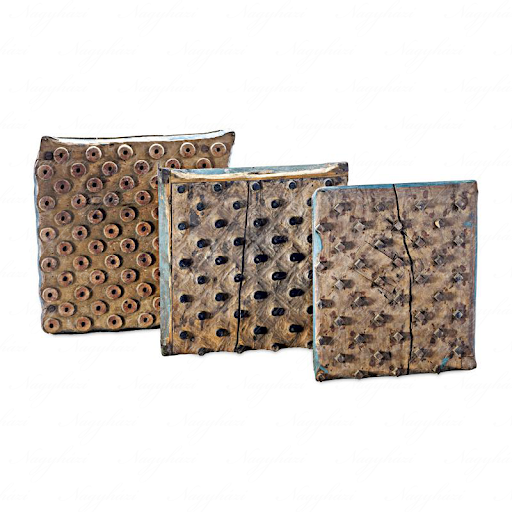
\includegraphics[width=\linewidth]{img/fábolkészült 01.png}
	  \caption{}
	\end{subfigure}
	\begin{subfigure}[b]{0.2\linewidth}
		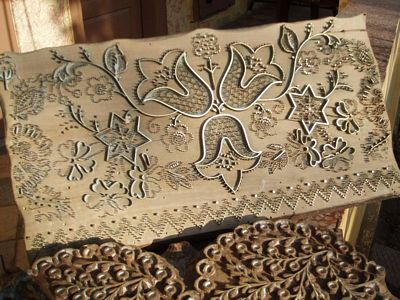
\includegraphics[width=\linewidth]{img/fémbőlkészült.jpg}
		\caption{}
	  \end{subfigure}
	  \begin{subfigure}[b]{0.15\linewidth}
		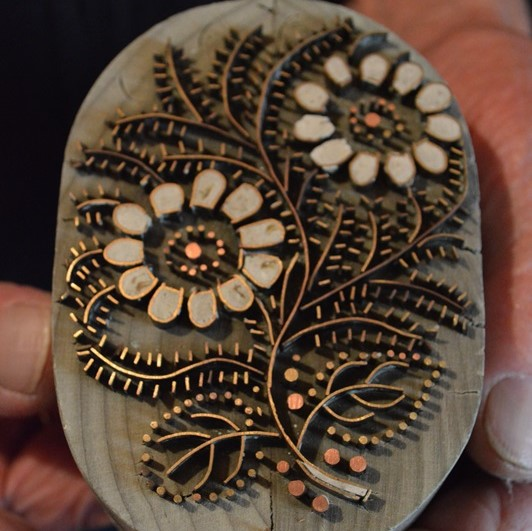
\includegraphics[width=\linewidth]{img/fémből készült 01.jpg}
		\caption{}
	  \end{subfigure}
	\caption{Nyomódúcok}
	\label{fig:duc}
  \end{figure}

%fábólkészült02  %fábolkészült01 %fémbölkészült %fémbölkészult 01
A fémből készített mintáknak a legfontosabb tartozéka az ún volt. A fémből készült minták nagyon időigényesek voltak. A mintákat úgy kezdik el megtervezni hogy elszőr papír terveket készítenek miután azt elfogadták a mintát elkezdi felrajzolni a minta fára és utána belakozza, hogy miközben készít ne mosódjon el rajt a minta, ritkább vagy bonyolultabb mintáknál a bekarcolják a mintafát, hogy pontosan helyezkedjenek el az elemek.
A minta dúcokra készített mintákhoz lapos vésőt ütögetve haladnak és közben beverik a lemezeket. Ha több szint szeretek volna alkalmazni akkor egy kiegészítő dúcot is készítettek a a kiegészítőmintáról.

Sok festő művész készített ekkor tálytt mintaterveket mit például a békéscsabai festő műhely tulajdonosa Sztaricskay Pál a ki régi kedvenc kézi mintáit elkészítette a gépi nyomáshoz is, aki még  gépi mintákat készített az Gál Gyula volt. Sok esetben ezeket a mintákat csak egy mesternek adták el.

\subsection{Alap minták}
%egyszerübb pontozott minta
Az öltözködés terén többnyire női ruhákon lehetett látni könnyed és nagyobb, egyszerűbb alap mintákat, formákat mint például virágók, levelek, apró pöttyök vagy geometrikus formák.
Ezek a minták ugyan úgy rá kerültek ágymenükre zsebkendőre, de terítőn is felehetők voltak.
A természeti motívumok mellet egyre jobban megjelentek és divatossá váltak a geometrikus formák is.
A kezdetekben egyszerű mintákat használtak (\ref{fig:egyszeruminta}. ábra) az idő előre haladtával váltak egyre bonyolultabbá és részletesebb ahogy azt a kor divatja és vevői igényei diktálták.

\begin{figure}[h!]
	\centering
	\includegraphics[width=0.55\textwidth]{img/egyszerübb pontozott minta.jpg}
	\caption{Egyszerű pontozott minta}
	\label{fig:egyszeruminta}
\end{figure}

\subsection{Minta fejlődés}
%sürübb minta 
A Minták olyan irányban fejlődtek tovább, hogy nem csak a már említett egyszerűbb minták voltak hanem  elkezdtek más művészeti területekről mintákat beemelni és azokat is tovább fejleszteni (\ref{fig:suruminta}. ábra).
Sokkal nagyon mintafákat készítettek sokkal sűrűbb és aprólékosabb virág, levél motívumokal. Megjelentek a családi címerek is a mintafákon vagy olyan mintát ahol már történtek szerepeltek mint például vallási jelenetek Ádám és Éva története vagy vadász jelenetek voltak megjelenítve az nem minden esetben volt tiszta hogy igazából miért is jelenítetek meg eseményeket. Pápán a 16. század közepe tájékán  készítettek hímzést utánzó kendő mintákat is. A többi városban mint például Gyula itt damasztszövéshez hasonló minta fát csináltak, Cegléden is az ottani mesterek készítettek szövést és hímzést ábrázoló mintákat.

\begin{figure}[h!]
	\centering
	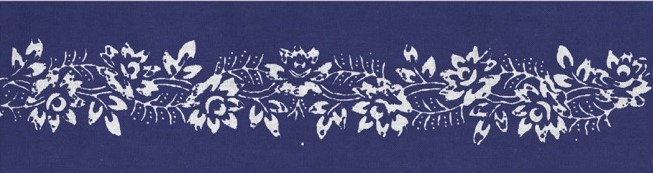
\includegraphics[width=0.55\textwidth]{img/sürübb minta.jpg}
	\caption{Sűrübb minta}
	\label{fig:suruminta}
\end{figure}

\subsection{Egyébb fő minták motívumok}
%levelek01 %virág 01
Fő motívumoknak lehetnek nevezni a kékfestészetben a virág ábrázolásokat vagy valamilyen fajta formáját.  
Ezek a mintaelemek teljes formájukban szoktak megjeleni vagy vonal ábrázolássl vagy egy két ponttal ábrázolták ezeke (\ref{fig:levelvirag}. ábra).
A virág ábrázolások jelentése a szeretetett, a hűséget jelképezte és  ezeket a gondolatokat fejezete ki formailag, változatos színvilága sajátos rezgéseket és érzések váltanak ki az emberekből.

\begin{figure}[h!]
	\centering
	\begin{subfigure}[b]{0.4\linewidth}
	  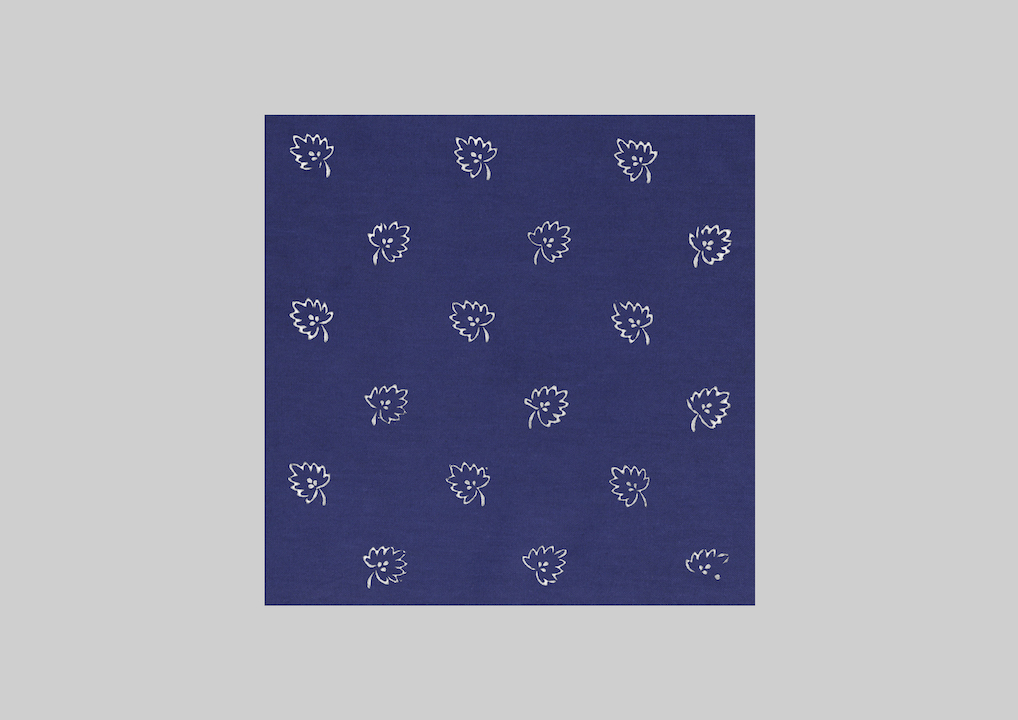
\includegraphics[width=\linewidth]{img/levél01.png}
	  \caption{}
	\end{subfigure}
	\begin{subfigure}[b]{0.43\linewidth}
	  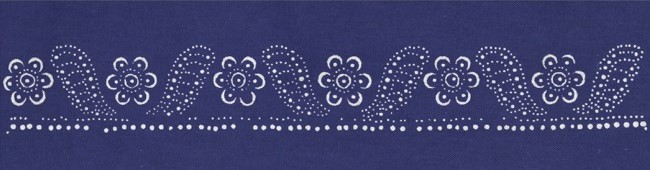
\includegraphics[width=\linewidth]{img/virág 01.jpg}
	  \caption{}
	\end{subfigure}
	\caption{Levél és virág motívumok}
	\label{fig:levelvirag}
  \end{figure}

\section{Hagyományos kékfestő műhelyek}
A Tolnai Kékfestő műhely Magyarország  egyik legrégebbi még ma is működő kékfestő műhely 1810-ben alpítoták.
Műhelyben még fellelhetők a régi eszközök az eredeti hagyományokat követik, még a mai napig a régi eszközökkel dolgoznak.
Motívumaikra jellemző, hogy csak is a régi családi mintafákat használják fel.
Ezekből a minta készletből több mint ötszáz darabbal rendelkezik a család.
Sajnos ezek a darabok nem pótólhatók mert sajnos hazákban évtizedek óta kihalt ez a mesterség, nincsenek már olyan mesterek akik a minta készítéssel foglalkoznak igy nincs nagyon lehetőség pótolni a tönkre 
ment darabokat.

\section{Kortás megoldások és adaptációk}

\subsection{Polgár Csaba}
Polgár Csaba(Budapest, 1942-03-19, Budapest, 2016-02-11) textílművész munkásságát nagy mértékben befolyásolta a kortárs modern művészet, korszerűséget mindigis komolyan vette, munkáiban előszerettetel mutatta meg a szabadság érzetét \cite{plogarcs}.

\begin{figure}[ht!]
	\centering
	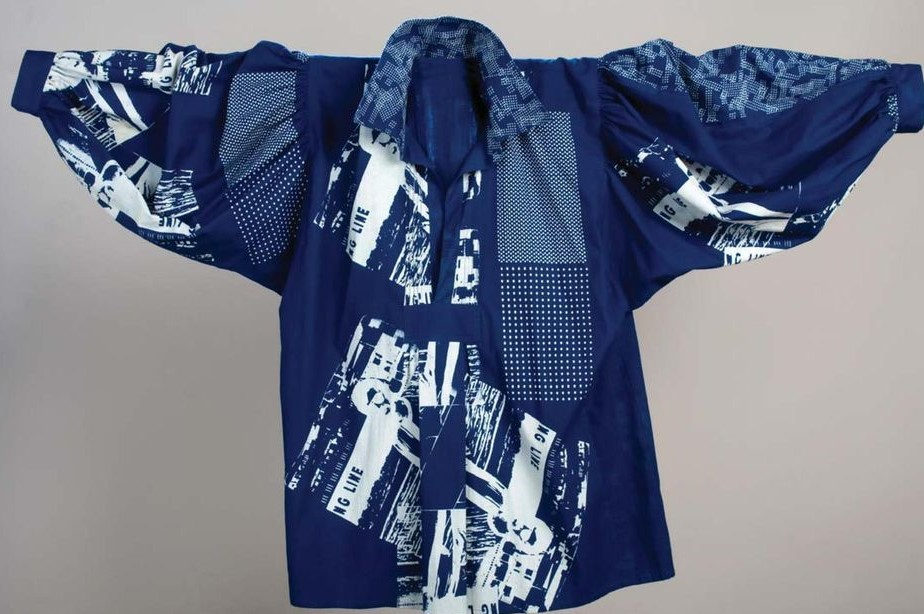
\includegraphics[width=0.55\textwidth]{img/quasi.jpg}
	\caption{Quasi kékfestő program - fényfestésnek - ing}
	\label{fig:quasi}
\end{figure}

Egy új művészeti technológiát fejlesztett ki amit fényfestésnek (\ref{fig:quasi}. ábra) vagy fakításnak nevezett el, ez a technika igazából a fotogramnak a fordítottja, folyamat röviden  a következő lépésekből áll, a festett anyag kikerül a napra akkor veszít a színéből, kitakarásokkal lehet szabályozni, hogy hol fakuljon jobban ezzel külömböző
mintákat hozva létre és a kékre festett alap anyagra dróthálókat teker és így rács szerű mintákat fakít ki belőle.
Az ő nevéhez fűződik a Quasi kékfestő program  a programban nem  kékfestő minta dúcokal állitoták elö a mintákat hanem szitával készítették el ezeket a kék anyagokra. Ennek a technikának az alkalmazása teszi lehetővé új textil karakter  létrehozását, de megmaradva a múltbeli alap technikáknál.

\subsection{Horváth Yoshihara Hanga} 
Horváth Yoshihara Hanga japánban élő textilművész fő kutatási területe \cite{hanga2010} a kékfestés hagyományos japán megfelelője a Shibori(\ref{fig:hyh}. ábra).

A munkái során tanulmányozta a növényi festési technikákat itt leginkább az indigóval való festés, színezés lehetőségeit. Kutatása kitért még a termesztési folyamatokra is amit japán tanulmányi uúa során Tokusimában végzett.

\begin{figure}[h!]
	\centering
	\begin{subfigure}[b]{0.3\linewidth}
	  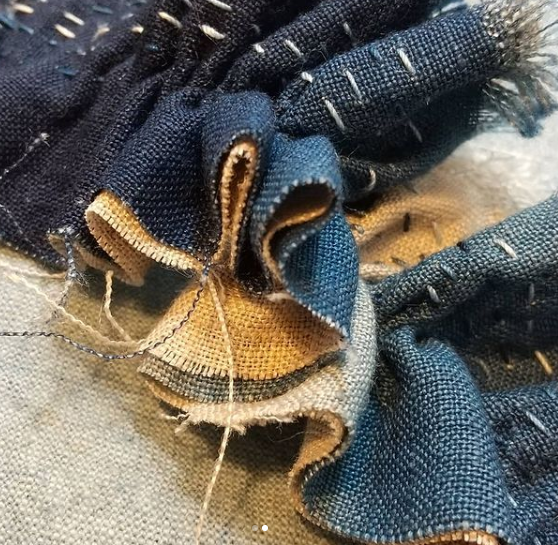
\includegraphics[width=\linewidth]{img/hh_01.png}
	  \caption{}
	\end{subfigure}
	\begin{subfigure}[b]{0.3\linewidth}
	  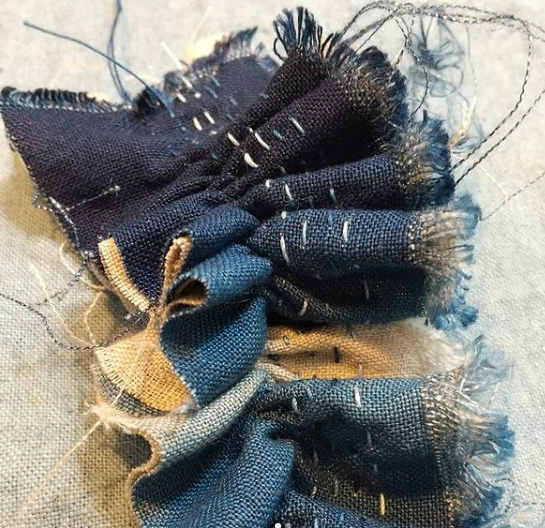
\includegraphics[width=\linewidth]{img/hh_02.png}
	  \caption{}
	\end{subfigure}
	\begin{subfigure}[b]{0.32\linewidth}
		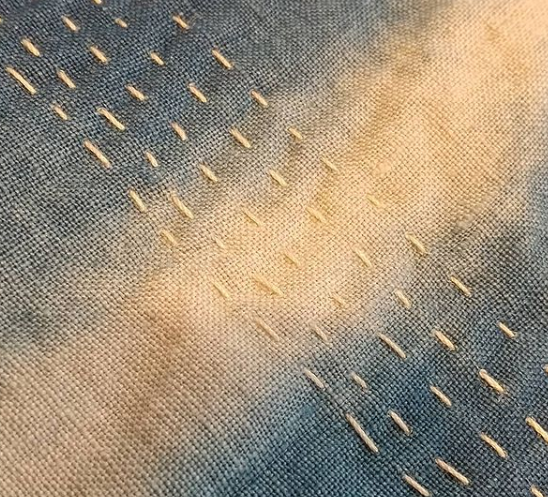
\includegraphics[width=\linewidth]{img/hh_3.png}
		\caption{}
	  \end{subfigure}
	\caption{Horváth Yoshihara Hanga Shibori munkái (forrás:\href{https://www.instagram.com/cicvarek1223}{instagram.com})}
	\label{fig:hyh}
  \end{figure}
\newpage
\subsection{Tóvaj Rozália}

\begin{figure}[ht!]
	\centering
	\begin{subfigure}[b]{0.3\linewidth}
	  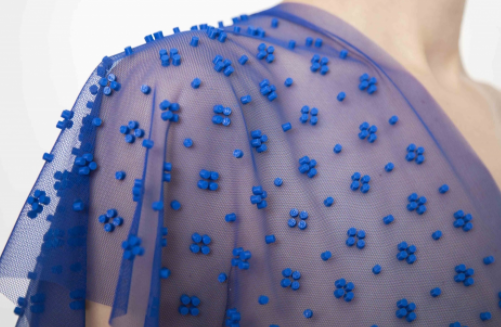
\includegraphics[width=\linewidth]{img/tr_01.png}
	  \caption{}
	\end{subfigure}
	\begin{subfigure}[b]{0.22\linewidth}
	  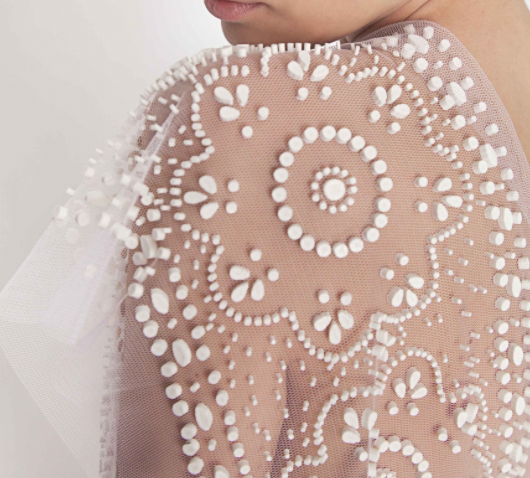
\includegraphics[width=\linewidth]{img/tr_02.png}
	  \caption{}
	\end{subfigure}
	\begin{subfigure}[b]{0.3\linewidth}
		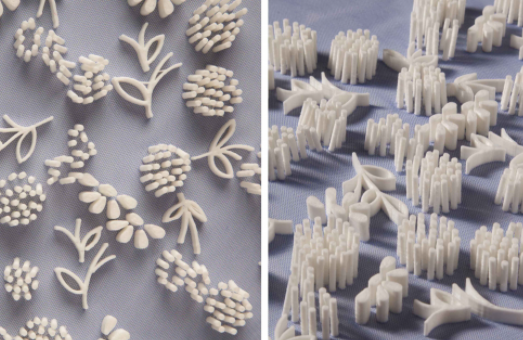
\includegraphics[width=\linewidth]{img/tr_03.png}
		\caption{}
	  \end{subfigure}
	\caption{Tóvaj Rozália 3D kékfestés}
	\label{fig:tr}
  \end{figure}

  Tóvaj Rozália mestermunkája \cite{tovaj2018} során azzal foglalkozott, hogy újra szerette volna gondolni a hagyományos kékfestést. A célja a gazadag kulturkincs és a mintarendszer tovább vitele a jelenkori technologiákkal. A végső eredmény az lett, hogy a hagyományos mintákat 3D nyomtatással készítette el lágy anyagokra így megidézve a hagyományos formai és minta világot.

\chapter{Összegzés} 
A szakdolgozatom irássa közben megismertem, hogy a természet mint eszköz és forrás hogyan valósul meg és ezek milyen hatással voltak/vannak az emberiségre milyen technikák, minták alakultak ki.
Ezeknek az ismerete új inspirációt adott és irányt adtak a saját mintakicsem bővitésére.

Megismerkedtem azokkal az alap módszerekkel amivel az ember felhasználta a természetes szineket és azt, hogy hogyan alakították ki, használták fel és hogy ez mely területeken fordult mind földrajzilag és művészetileg.
Ezek a technikák a legfőképpen a textil művészetekben valósulnak meg az alapanyagok megfestésével, színezésével.

A dolgozat alatt két fő régiót vizsgáltam meg Ázsiát és Európát ezeken belül is elsődlegesen Japánt és Magyarországot. Japánban a shibori technika míg magyarországon  a kékfestő volt.

E két technika bemutatása során meg ismerkedtem a folyamatokkal melyekkel a textíliákat színezik és ahogy ezeken kialakítják a mintázattokat.
Bemutattam olyan kortás művészeket akiki  két hagyományos kézműves technika álltal inspirálódtak és saját adaptációt valósítottak meg.




%\printbibliography
\bibliography{thesis}

% \renewcommand{\appendixname}{Függelék}  % különben "Appendix"-et ír
% \appendix
% \chapter{Mellékletek listája}

\end{document}